\documentclass[10pt,a4paper]{article}
\usepackage[utf8]{inputenc}
\usepackage[margin=2cm]{geometry}
\usepackage{amsmath}
\usepackage{amsfonts}
\usepackage{multicol}
\usepackage{amssymb}
\usepackage{graphicx}
\usepackage{tikz}

\usepackage[uprightgreeks,frenchstyle,light,fulloldstylenums,veryoldstyle]{kpfonts}
%\usepackage[small]{eulervm}
%\usepackage[osf,sc]{mathpazo}

\begin{document}
\centering
\begin{multicols}{3}

\par \textit{Fig 1}

\par \begin{tikzpicture}[rotate=180, scale=1.4]
	\draw [shift={(-1.651,-2.108)}]  plot[domain=0.141:0.906,variable=\t]({1.*2.678*cos(\t r)+0.*2.677*sin(\t r)},{0.*2.678*cos(\t r)+1.*2.678*sin(\t r)});
	\draw [shift={(1,2.484)}]  plot[domain=4.330:5.095,variable=\t]({1.*2.678*cos(\t r)+0.*2.678*sin(\t r)},{0.*2.678*cos(\t r)+1.*2.678*sin(\t r)});
	\draw [shift={(3.651,-2.108)}]  plot[domain=2.235:3.001,variable=\t]({1.*2.678*cos(\t r)+0.*2.678*sin(\t r)},{0.*2.678*cos(\t r)+1.*2.678*sin(\t r)});
	\draw (0,0) node [below right] {\small $C$};
	\draw (2,0) node [below left] {\small $B$};
	\draw (1,-1.732) node [above] {\small $A$};
\end{tikzpicture}

\vfill
\null

\columnbreak
	
\par \textit{Fig 2}

\par 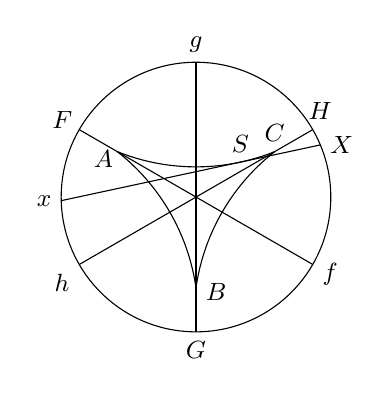
\begin{tikzpicture}
	\draw [shift={(-1.651,-2.108)}]  plot[domain=0.141:0.906,variable=\t]({1.*2.678*cos(\t r)+0.*2.677*sin(\t r)},{0.*2.678*cos(\t r)+1.*2.678*sin(\t r)});
	\draw [shift={(1,2.484)}]  plot[domain=4.330:5.095,variable=\t]({1.*2.678*cos(\t r)+0.*2.678*sin(\t r)},{0.*2.678*cos(\t r)+1.*2.678*sin(\t r)});
	\draw [shift={(3.651,-2.108)}]  plot[domain=2.235:3.001,variable=\t]({1.*2.678*cos(\t r)+0.*2.678*sin(\t r)},{0.*2.678*cos(\t r)+1.*2.678*sin(\t r)});
	\draw (1,-0.577) circle (1.712cm);
	\draw (1,1.135)-- (1,-2.290);
	\draw (2.483,-1.433)-- (-0.483,0.279);
	\draw (-0.483,-1.434)-- (2.483,0.279);
	\draw (2.579,0.085)-- (-0.712,-0.623);
	\draw (0,0) node [below left, yshift=4pt, xshift=2pt] {\small $A$};
	\draw (2,0) node [above] {\small $C$};
	\draw (1,-1.732) node [below right, yshift=5pt] {\small $B$};
	\draw (1,1.135) node [above] {\small $g$};
	\draw (2.483,0.279) node [above right, xshift=-5pt] {\small $H$};
	\draw (2.483,-1.434) node [below right, yshift=4pt] {\small $f$};
	\draw (-0.483,0.279) node [above left, yshift=-3pt, xshift=1pt] {\small $F$};
	\draw (-0.483,-1.434) node [below left] {\small $h$};
	\draw (1,-2.290) node [below] {\small $G$};
	\draw (1.563,-0.134) node [above] {\small $S$};
	\draw (2.579,0.085) node [right] {\small $X$};
	\draw (-0.712,-0.623) node [left] {\small $x$};
\end{tikzpicture}

\par \textit{Fig 3}

\par 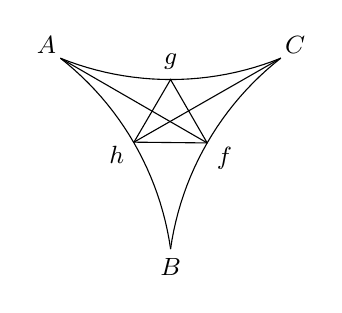
\begin{tikzpicture}[scale=1.4]
	\draw [shift={(-1.651,-2.108)}]  plot[domain=0.141:0.906,variable=\t]({1.*2.678*cos(\t r)+0.*2.677*sin(\t r)},{0.*2.678*cos(\t r)+1.*2.678*sin(\t r)});
	\draw [shift={(1,2.484)}]  plot[domain=4.330:5.095,variable=\t]({1.*2.678*cos(\t r)+0.*2.678*sin(\t r)},{0.*2.678*cos(\t r)+1.*2.678*sin(\t r)});
	\draw [shift={(3.651,-2.108)}]  plot[domain=2.235:3.001,variable=\t]({1.*2.678*cos(\t r)+0.*2.678*sin(\t r)},{0.*2.678*cos(\t r)+1.*2.678*sin(\t r)});
	\draw (0,0) node [above left, xshift=2pt, yshift=-2pt] {\small $A$};
	\draw (2,0) node [above right, xshift=-2pt, yshift=-2pt] {\small $C$};
	\draw (1,-1.732) node [below] {\small $B$};
	\draw (1,-0.194) -- (1.332,-0.769) -- (0.668,-0.762) -- cycle;
	\draw (0,0) -- (1.332,-0.769);
	\draw (2,0) -- (0.668,-0.762);
	\draw (1,-0.194) node [above] {\small $g$};
	\draw (1.332,-0.769) node [below right, yshift=2pt] {\small $f$};
	\draw (0.668,-0.762) node [below left, yshift=2pt] {\small $h$};
\end{tikzpicture}

\end{multicols}
\vfill 
\begin{multicols}{3}
\par \textit{Fig 4}

\par 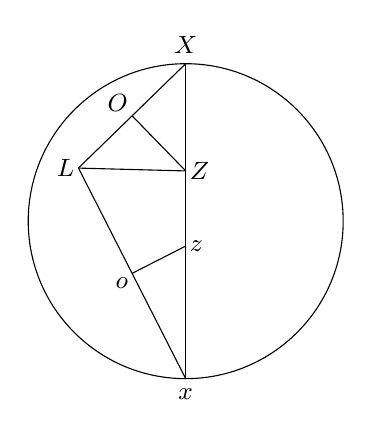
\begin{tikzpicture}
	\draw (0,0) circle (2cm);
	\draw (0,-2)-- (0,2);
	\draw (0,-2) -- (-1.362,0.675)-- (0,2);
	\draw (0,0.638)-- (-1.361,0.674);
	\draw (0,0.638)-- (-0.680,1.337);
	\draw (-0.681,-0.663)-- (0,-0.316);
	\draw (0,2) node [above] {\small $X$};
	\draw (0,-2) node [below] {\small $x$};
	\draw (-1.362,0.674) node [left, xshift=2pt] {\small $L$};
	\draw (-0.680,-0.662) node [below left, xshift=2pt, yshift=2pt] {\small $o$};
	\draw (-0.680,1.337) node [above left, xshift=2pt, yshift=-2pt] {\small $O$};
	\draw (0,0.637) node [right, xshift=-2pt] {\small $Z$};
	\draw (0,-0.316) node [right, xshift=-2pt] {\small $z$};
\end{tikzpicture}

\par \textit{Fig 5}

\par 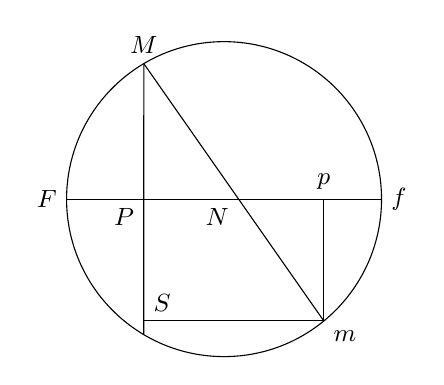
\begin{tikzpicture}
	\draw (0,0) circle (2cm);
	\draw (-2,0)-- (2,0);
	\draw (-1.019,1.721)-- (1.267,-1.547);
	\draw (-1.019,1.721)-- (-1.020,-1.720);
	\draw (-1.019,-1.547)-- (1.267,-1.547);
	\draw (1.267,-1.547)-- (1.267,0.);
	\draw (-1.0192,1.720) node [above] {\small $M$};
	\draw (-2.,0.) node [left] {\small $F$};
	\draw (2.,0.) node [right] {\small $f$};
	\draw (-1.0193,0.) node [below left] {\small $P$};
	%\draw (-1.0193,-1.721) node [above] {\small $e$};
	\draw (1.267,-1.547) node [below right] {\small $m$};
	\draw (0.184,0.) node [below left] {\small $N$};
	\draw (1.267,0.) node [above] {\small $p$};
	\draw (-1.019,-1.547) node [above right] {\small $S$};
\end{tikzpicture}

\vfill 
\null
\columnbreak

\par \textit{Fig 6}
\par 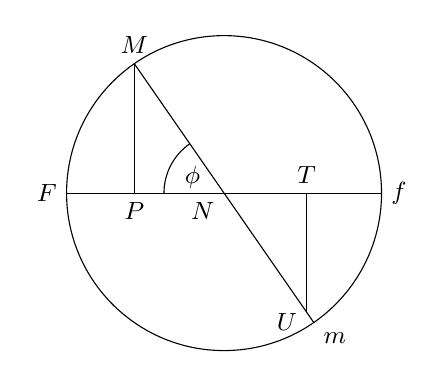
\begin{tikzpicture}
	\draw (124.73955121402813:0.7631107015839075) arc (124.73955121402813:180.:0.7631107015839075);
	\draw (0,0) circle (2cm);
	\draw (-1.1396938257701044,1.643501744295242)-- (1.1396938257701044,-1.643501744295242);
	\draw (1.0499141426476895,-1.5140344588914103)-- (1.0499141426476895,0.);
	\draw (-1.1396938257701044,0.)-- (-1.1396938257701044,1.643501744295242);
	\draw (-2,0)-- (2,0);
	
	\draw (0,0) node [below left] {\small $N$};
	\draw (-2,0) node [left] {\small $F$};
	\draw (2,0) node [right] {\small $f$};
	\draw (-1.1396938257701044,1.643501744295242) node [above] {\small $M$};
	\draw (1.1396938257701044,-1.643501744295242) node [below right] {\small $m$};
	\draw (-1.1396938257701044,0.) node [below] {\small $P$};
	\draw (1.0499141426476895,-1.5140344588914103) node [below left,yshift=3pt] {\small $U$};
	\draw (1.0499141426476895,0.) node [above] {\small $T$};
	\draw (-0.4,0.2) node {\small $\phi$};
\end{tikzpicture}

\end{multicols}
\vfill 
\begin{multicols}{3}

\par \textit{Fig 7}

\par 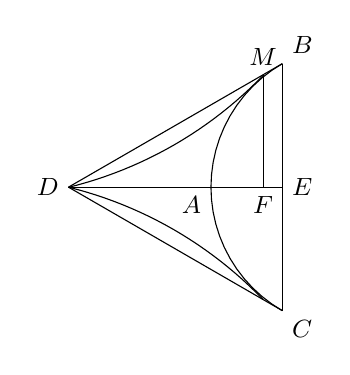
\begin{tikzpicture}
	\draw (-1.592,0.)-- (1.123,1.568);
	\draw (1.123,1.568)-- (1.123,-1.568);
	\draw (1.123,-1.568)-- (-1.592,0);
	\draw [shift={(2.028,0)}] plot[domain=2.094:4.1891,variable=\t]({1.*1.8107218179771583*cos(\t r)+0.*1.8107218179771583*sin(\t r)},{0.*1.8107218179771583*cos(\t r)+1.*1.8107218179771583*sin(\t r)});
	\draw [shift={(-2.82,4.994)}]  plot[domain=4.954772812894923:5.517202699071053,variable=\t]({1.*5.145122693791882*cos(\t r)+0.*5.145122693791882*sin(\t r)},{0.*5.145122693791882*cos(\t r)+1.*5.145122693791882*sin(\t r)});
	\draw [shift={(-2.8279022506987714,-4.994723411507955)}]  plot[domain=4.954772812894923:5.517202699071053,variable=\t]({1.*5.145122693791882*cos(\t r)+0.*5.145122693791882*sin(\t r)},{0.*5.145122693791882*cos(\t r)+-1.*5.145122693791882*sin(\t r)});
	\draw (-1.593,0)-- (1.124,0);
	\draw (0.880,1.427) -- (0.880,0);
	\draw (1.123,1.568) node [above right] {\small $B$};
	\draw (1.123,-1.568) node [below right] {\small $C$};
	\draw (-1.592,0) node [left] {\small $D$};
	\draw (1.123,0) node [right] {\small $E$};
	\draw (0.217,0) node [below left] {\small $A$};
	\draw (0.880,1.427) node [above] {\small $M$};
	\draw (0.880,0) node [below] {\small $F$};
\end{tikzpicture}

\vfill 
\null
\columnbreak
\null

\vfill 
\null
\columnbreak
\null
\end{multicols}

\end{document}